\chapter{The Abbé’s Chamber}

After having passed with tolerable ease through the subterranean
passage, which, however, did not admit of their holding themselves
erect, the two friends reached the further end of the corridor, into
which the abbé’s cell opened; from that point the passage became much
narrower, and barely permitted one to creep through on hands and knees.
The floor of the abbé’s cell was paved, and it had been by raising one
of the stones in the most obscure corner that Faria had been able to
commence the laborious task of which Dantès had witnessed the
completion.

As he entered the chamber of his friend, Dantès cast around one eager
and searching glance in quest of the expected marvels, but nothing more
than common met his view.

“It is well,” said the abbé; “we have some hours before us—it is now
just a quarter past twelve o’clock.” Instinctively Dantès turned round
to observe by what watch or clock the abbé had been able so accurately
to specify the hour.

“Look at this ray of light which enters by my window,” said the abbé,
“and then observe the lines traced on the wall. Well, by means of these
lines, which are in accordance with the double motion of the earth, and
the ellipse it describes round the sun, I am enabled to ascertain the
precise hour with more minuteness than if I possessed a watch; for that
might be broken or deranged in its movements, while the sun and earth
never vary in their appointed paths.”

This last explanation was wholly lost upon Dantès, who had always
imagined, from seeing the sun rise from behind the mountains and set in
the Mediterranean, that it moved, and not the earth. A double movement
of the globe he inhabited, and of which he could feel nothing, appeared
to him perfectly impossible. Each word that fell from his companion’s
lips seemed fraught with the mysteries of science, as worthy of digging
out as the gold and diamonds in the mines of Guzerat and Golconda,
which he could just recollect having visited during a voyage made in
his earliest youth.

“Come,” said he to the abbé, “I am anxious to see your treasures.”

The abbé smiled, and, proceeding to the disused fireplace, raised, by
the help of his chisel, a long stone, which had doubtless been the
hearth, beneath which was a cavity of considerable depth, serving as a
safe depository of the articles mentioned to Dantès.

\begin{figure}[ht]
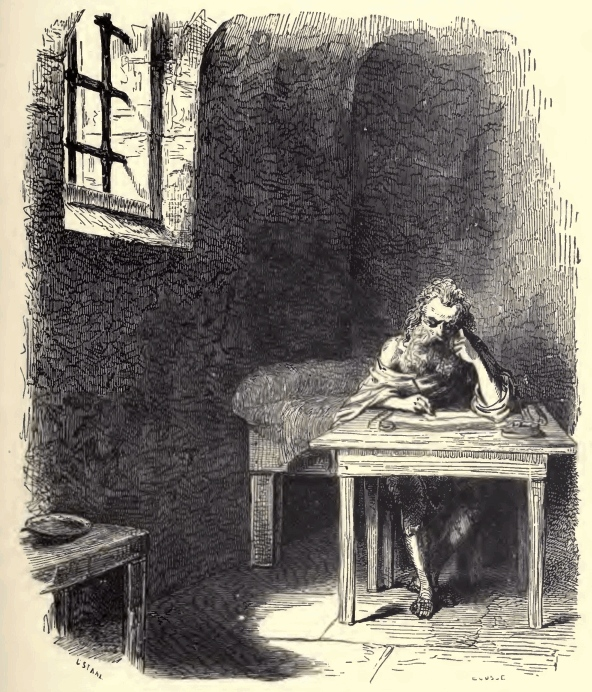
\includegraphics[width=\textwidth]{0213m.jpg}
\end{figure}

“What do you wish to see first?” asked the abbé.

“Oh, your great work on the monarchy of Italy!”

Faria then drew forth from his hiding-place three or four rolls of
linen, laid one over the other, like folds of papyrus. These rolls
consisted of slips of cloth about four inches wide and eighteen long;
they were all carefully numbered and closely covered with writing, so
legible that Dantès could easily read it, as well as make out the
sense—it being in Italian, a language he, as a Provençal, perfectly
understood.

“There,” said he, “there is the work complete. I wrote the word \textit{finis}
at the end of the sixty-eighth strip about a week ago. I have torn up
two of my shirts, and as many handkerchiefs as I was master of, to
complete the precious pages. Should I ever get out of prison and find
in all Italy a printer courageous enough to publish what I have
composed, my literary reputation is forever secured.”

“I see,” answered Dantès. “Now let me behold the curious pens with
which you have written your work.”

“Look!” said Faria, showing to the young man a slender stick about six
inches long, and much resembling the size of the handle of a fine
painting-brush, to the end of which was tied, by a piece of thread, one
of those cartilages of which the abbé had before spoken to Dantès; it
was pointed, and divided at the nib like an ordinary pen. Dantès
examined it with intense admiration, then looked around to see the
instrument with which it had been shaped so correctly into form.

“Ah, yes,” said Faria; “the penknife. That’s my masterpiece. I made it,
as well as this larger knife, out of an old iron candlestick.” The
penknife was sharp and keen as a razor; as for the other knife, it
would serve a double purpose, and with it one could cut and thrust.

Dantès examined the various articles shown to him with the same
attention that he had bestowed on the curiosities and strange tools
exhibited in the shops at Marseilles as the works of the savages in the
South Seas from whence they had been brought by the different trading
vessels.

“As for the ink,” said Faria, “I told you how I managed to obtain
that—and I only just make it from time to time, as I require it.”

“One thing still puzzles me,” observed Dantès, “and that is how you
managed to do all this by daylight?”

“I worked at night also,” replied Faria.

“Night!—why, for Heaven’s sake, are your eyes like cats’, that you can
see to work in the dark?”

“Indeed they are not; but God has supplied man with the intelligence
that enables him to overcome the limitations of natural conditions. I
furnished myself with a light.”

“You did? Pray tell me how.”

“I separated the fat from the meat served to me, melted it, and so made
oil—here is my lamp.” So saying, the abbé exhibited a sort of torch
very similar to those used in public illuminations.

“But how do you procure a light?”

“Oh, here are two flints and a piece of burnt linen.”

“And matches?”

“I pretended that I had a disorder of the skin, and asked for a little
sulphur, which was readily supplied.”

Dantès laid the different things he had been looking at on the table,
and stood with his head drooping on his breast, as though overwhelmed
by the perseverance and strength of Faria’s mind.

\begin{figure}[ht]
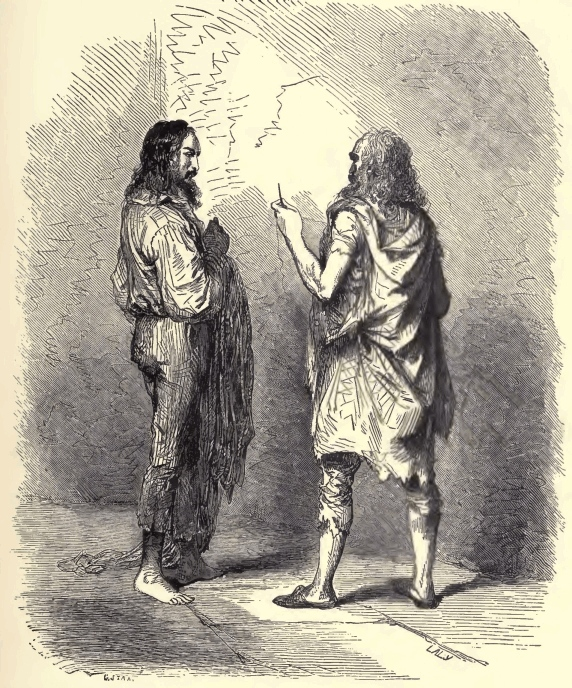
\includegraphics[width=\textwidth]{0215m.jpg}
\end{figure}

“You have not seen all yet,” continued Faria, “for I did not think it
wise to trust all my treasures in the same hiding-place. Let us shut
this one up.” They put the stone back in its place; the abbé sprinkled
a little dust over it to conceal the traces of its having been removed,
rubbed his foot well on it to make it assume the same appearance as the
other, and then, going towards his bed, he removed it from the spot it
stood in. Behind the head of the bed, and concealed by a stone fitting
in so closely as to defy all suspicion, was a hollow space, and in this
space a ladder of cords between twenty-five and thirty feet in length.
Dantès closely and eagerly examined it; he found it firm, solid, and
compact enough to bear any weight.

“Who supplied you with the materials for making this wonderful work?”

“I tore up several of my shirts, and ripped out the seams in the sheets
of my bed, during my three years’ imprisonment at Fenestrelle; and when
I was removed to the Château d’If, I managed to bring the ravellings
with me, so that I have been able to finish my work here.”

“And was it not discovered that your sheets were unhemmed?”

“Oh, no, for when I had taken out the thread I required, I hemmed the
edges over again.”

“With what?”

“With this needle,” said the abbé, as, opening his ragged vestments, he
showed Dantès a long, sharp fish-bone, with a small perforated eye for
the thread, a small portion of which still remained in it.

“I once thought,” continued Faria, “of removing these iron bars, and
letting myself down from the window, which, as you see, is somewhat
wider than yours, although I should have enlarged it still more
preparatory to my flight; however, I discovered that I should merely
have dropped into a sort of inner court, and I therefore renounced the
project altogether as too full of risk and danger. Nevertheless, I
carefully preserved my ladder against one of those unforeseen
opportunities of which I spoke just now, and which sudden chance
frequently brings about.”

While affecting to be deeply engaged in examining the ladder, the mind
of Dantès was, in fact, busily occupied by the idea that a person so
intelligent, ingenious, and clear-sighted as the abbé might probably be
able to solve the dark mystery of his own misfortunes, where he himself
could see nothing.

“What are you thinking of?” asked the abbé smilingly, imputing the deep
abstraction in which his visitor was plunged to the excess of his awe
and wonder.

“I was reflecting, in the first place,” replied Dantès, “upon the
enormous degree of intelligence and ability you must have employed to
reach the high perfection to which you have attained. What would you
not have accomplished if you had been free?”

“Possibly nothing at all; the overflow of my brain would probably, in a
state of freedom, have evaporated in a thousand follies; misfortune is
needed to bring to light the treasures of the human intellect.
Compression is needed to explode gunpowder. Captivity has brought my
mental faculties to a focus; and you are well aware that from the
collision of clouds electricity is produced—from electricity,
lightning, from lightning, illumination.”

“No,” replied Dantès. “I know nothing. Some of your words are to me
quite empty of meaning. You must be blessed indeed to possess the
knowledge you have.”

The abbé smiled. “Well,” said he, “but you had another subject for your
thoughts; did you not say so just now?”

“I did!”

“You have told me as yet but one of them—let me hear the other.”

“It was this,—that while you had related to me all the particulars of
your past life, you were perfectly unacquainted with mine.”

“Your life, my young friend, has not been of sufficient length to admit
of your having passed through any very important events.”

“It has been long enough to inflict on me a great and undeserved
misfortune. I would fain fix the source of it on man that I may no
longer vent reproaches upon Heaven.”

“Then you profess ignorance of the crime with which you are charged?”

“I do, indeed; and this I swear by the two beings most dear to me upon
earth,—my father and Mercédès.”

“Come,” said the abbé, closing his hiding-place, and pushing the bed
back to its original situation, “let me hear your story.”

Dantès obeyed, and commenced what he called his history, but which
consisted only of the account of a voyage to India, and two or three
voyages to the Levant, until he arrived at the recital of his last
cruise, with the death of Captain Leclere, and the receipt of a packet
to be delivered by himself to the grand marshal; his interview with
that personage, and his receiving, in place of the packet brought, a
letter addressed to a Monsieur Noirtier—his arrival at Marseilles, and
interview with his father—his affection for Mercédès, and their nuptual
feast—his arrest and subsequent examination, his temporary detention at
the Palais de Justice, and his final imprisonment in the Château d’If.
From this point everything was a blank to Dantès—he knew nothing more,
not even the length of time he had been imprisoned. His recital
finished, the abbé reflected long and earnestly.

“There is,” said he, at the end of his meditations, “a clever maxim,
which bears upon what I was saying to you some little while ago, and
that is, that unless wicked ideas take root in a naturally depraved
mind, human nature, in a right and wholesome state, revolts at crime.
Still, from an artificial civilization have originated wants, vices,
and false tastes, which occasionally become so powerful as to stifle
within us all good feelings, and ultimately to lead us into guilt and
wickedness. From this view of things, then, comes the axiom that if you
visit to discover the author of any bad action, seek first to discover
the person to whom the perpetration of that bad action could be in any
way advantageous. Now, to apply it in your case,—to whom could your
disappearance have been serviceable?”

“To no one, by Heaven! I was a very insignificant person.”

“Do not speak thus, for your reply evinces neither logic nor
philosophy; everything is relative, my dear young friend, from the king
who stands in the way of his successor, to the employee who keeps his
rival out of a place. Now, in the event of the king’s death, his
successor inherits a crown,—when the employee dies, the supernumerary
steps into his shoes, and receives his salary of twelve thousand
livres. Well, these twelve thousand livres are his civil list, and are
as essential to him as the twelve millions of a king. Everyone, from
the highest to the lowest degree, has his place on the social ladder,
and is beset by stormy passions and conflicting interests, as in
Descartes’ theory of pressure and impulsion. But these forces increase
as we go higher, so that we have a spiral which in defiance of reason
rests upon the apex and not on the base. Now let us return to your
particular world. You say you were on the point of being made captain
of the \textit{Pharaon}?”

“Yes.”

“And about to become the husband of a young and lovely girl?”

“Yes.”

“Now, could anyone have had any interest in preventing the
accomplishment of these two things? But let us first settle the
question as to its being the interest of anyone to hinder you from
being captain of the \textit{Pharaon}. What say you?”

“I cannot believe such was the case. I was generally liked on board,
and had the sailors possessed the right of selecting a captain
themselves, I feel convinced their choice would have fallen on me.
There was only one person among the crew who had any feeling of
ill-will towards me. I had quarelled with him some time previously, and
had even challenged him to fight me; but he refused.”

“Now we are getting on. And what was this man’s name?”

“Danglars.”

“What rank did he hold on board?”

“He was supercargo.”

“And had you been captain, should you have retained him in his
employment?”

“Not if the choice had remained with me, for I had frequently observed
inaccuracies in his accounts.”

“Good again! Now then, tell me, was any person present during your last
conversation with Captain Leclere?”

“No; we were quite alone.”

“Could your conversation have been overheard by anyone?”

“It might, for the cabin door was open—and—stay; now I
recollect,—Danglars himself passed by just as Captain Leclere was
giving me the packet for the grand marshal.”

“That’s better,” cried the abbé; “now we are on the right scent. Did
you take anybody with you when you put into the port of Elba?”

“Nobody.”

“Somebody there received your packet, and gave you a letter in place of
it, I think?”

“Yes; the grand marshal did.”

“And what did you do with that letter?”

“Put it into my portfolio.”

“You had your portfolio with you, then? Now, how could a sailor find
room in his pocket for a portfolio large enough to contain an official
letter?”

“You are right; it was left on board.”

“Then it was not till your return to the ship that you put the letter
in the portfolio?”

“No.”

“And what did you do with this same letter while returning from
Porto-Ferrajo to the vessel?”

“I carried it in my hand.”

“So that when you went on board the \textit{Pharaon}, everybody could see that
you held a letter in your hand?”

“Yes.”

“Danglars, as well as the rest?”

“Danglars, as well as others.”

“Now, listen to me, and try to recall every circumstance attending your
arrest. Do you recollect the words in which the information against you
was formulated?”

“Oh yes, I read it over three times, and the words sank deeply into my
memory.”

“Repeat it to me.”

Dantès paused a moment, then said, “This is it, word for word: ‘The
king’s attorney is informed by a friend to the throne and religion,
that one Edmond Dantès, mate on board the \textit{Pharaon}, this day arrived
from Smyrna, after having touched at Naples and Porto-Ferrajo, has been
intrusted by Murat with a packet for the usurper; again, by the
usurper, with a letter for the Bonapartist Club in Paris. This proof of
his guilt may be procured by his immediate arrest, as the letter will
be found either about his person, at his father’s residence, or in his
cabin on board the \textit{Pharaon}.’”

The abbé shrugged his shoulders. “The thing is clear as day,” said he;
“and you must have had a very confiding nature, as well as a good
heart, not to have suspected the origin of the whole affair.”

“Do you really think so? Ah, that would indeed be infamous.”

“How did Danglars usually write?”

“In a handsome, running hand.”

“And how was the anonymous letter written?”

“Backhanded.”

Again the abbé smiled. “Disguised.”

“It was very boldly written, if disguised.”

“Stop a bit,” said the abbé, taking up what he called his pen, and,
after dipping it into the ink, he wrote on a piece of prepared linen,
with his left hand, the first two or three words of the accusation.
Dantès drew back, and gazed on the abbé with a sensation almost
amounting to terror.

“How very astonishing!” cried he at length. “Why your writing exactly
resembles that of the accusation.”

“Simply because that accusation had been written with the left hand;
and I have noticed that——”

“What?”

“That while the writing of different persons done with the right hand
varies, that performed with the left hand is invariably uniform.”

“You have evidently seen and observed everything.”

“Let us proceed.”

“Oh, yes, yes!”

“Now as regards the second question.”

“I am listening.”

“Was there any person whose interest it was to prevent your marriage
with Mercédès?”

“Yes; a young man who loved her.”

“And his name was——”

“Fernand.”

“That is a Spanish name, I think?”

“He was a Catalan.”

“You imagine him capable of writing the letter?”

“Oh, no; he would more likely have got rid of me by sticking a knife
into me.”

“That is in strict accordance with the Spanish character; an
assassination they will unhesitatingly commit, but an act of cowardice,
never.”

“Besides,” said Dantès, “the various circumstances mentioned in the
letter were wholly unknown to him.”

“You had never spoken of them yourself to anyone?”

“To no one.”

“Not even to your mistress?”

“No, not even to my betrothed.”

“Then it is Danglars.”

“I feel quite sure of it now.”

“Wait a little. Pray, was Danglars acquainted with Fernand?”

“No—yes, he was. Now I recollect——”

“What?”

“To have seen them both sitting at table together under an arbor at
Père Pamphile’s the evening before the day fixed for my wedding. They
were in earnest conversation. Danglars was joking in a friendly way,
but Fernand looked pale and agitated.”

“Were they alone?”

“There was a third person with them whom I knew perfectly well, and who
had, in all probability made their acquaintance; he was a tailor named
Caderousse, but he was very drunk. Stay!—stay!—How strange that it
should not have occurred to me before! Now I remember quite well, that
on the table round which they were sitting were pens, ink, and paper.
Oh, the heartless, treacherous scoundrels!” exclaimed Dantès, pressing
his hand to his throbbing brows.

“Is there anything else I can assist you in discovering, besides the
villany of your friends?” inquired the abbé with a laugh.

“Yes, yes,” replied Dantès eagerly; “I would beg of you, who see so
completely to the depths of things, and to whom the greatest mystery
seems but an easy riddle, to explain to me how it was that I underwent
no second examination, was never brought to trial, and, above all, was
condemned without ever having had sentence passed on me?”

“That is altogether a different and more serious matter,” responded the
abbé. “The ways of justice are frequently too dark and mysterious to be
easily penetrated. All we have hitherto done in the matter has been
child’s play. If you wish me to enter upon the more difficult part of
the business, you must assist me by the most minute information on
every point.”

“Pray ask me whatever questions you please; for, in good truth, you see
more clearly into my life than I do myself.”

“In the first place, then, who examined you,—the king’s attorney, his
deputy, or a magistrate?”

“The deputy.”

“Was he young or old?”

“About six or seven-and-twenty years of age, I should say.”

“So,” answered the abbé. “Old enough to be ambitious, but too young to
be corrupt. And how did he treat you?”

“With more of mildness than severity.”

“Did you tell him your whole story?”

“I did.”

“And did his conduct change at all in the course of your examination?”

“He did appear much disturbed when he read the letter that had brought
me into this scrape. He seemed quite overcome by my misfortune.”

“By your misfortune?”

“Yes.”

“Then you feel quite sure that it was your misfortune he deplored?”

“He gave me one great proof of his sympathy, at any rate.”

“And that?”

“He burnt the sole evidence that could at all have criminated me.”

“What? the accusation?”

“No; the letter.”

“Are you sure?”

“I saw it done.”

“That alters the case. This man might, after all, be a greater
scoundrel than you have thought possible.”

“Upon my word,” said Dantès, “you make me shudder. Is the world filled
with tigers and crocodiles?”

“Yes; and remember that two-legged tigers and crocodiles are more
dangerous than the others.”

“Never mind; let us go on.”

“With all my heart! You tell me he burned the letter?”

“He did; saying at the same time, ‘You see I thus destroy the only
proof existing against you.’”

“This action is somewhat too sublime to be natural.”

“You think so?”

“I am sure of it. To whom was this letter addressed?”

“To M. Noirtier, Rue Coq-Héron, No. 13, Paris.”

“Now can you conceive of any interest that your heroic deputy could
possibly have had in the destruction of that letter?”

“Why, it is not altogether impossible he might have had, for he made me
promise several times never to speak of that letter to anyone, assuring
me he so advised me for my own interest; and, more than this, he
insisted on my taking a solemn oath never to utter the name mentioned
in the address.”

“Noirtier!” repeated the abbé; “Noirtier!—I knew a person of that name
at the court of the Queen of Etruria,—a Noirtier, who had been a
Girondin during the Revolution! What was your deputy called?”

“De Villefort!” The abbé burst into a fit of laughter, while Dantès
gazed on him in utter astonishment.

“What ails you?” said he at length.

“Do you see that ray of sunlight?”

“I do.”

“Well, the whole thing is more clear to me than that sunbeam is to you.
Poor fellow! poor young man! And you tell me this magistrate expressed
great sympathy and commiseration for you?”

“He did.”

“And the worthy man destroyed your compromising letter?”

“Yes.”

“And then made you swear never to utter the name of Noirtier?”

“Yes.”

“Why, you poor short-sighted simpleton, can you not guess who this
Noirtier was, whose very name he was so careful to keep concealed? This
Noirtier was his father!”

Had a thunderbolt fallen at the feet of Dantès, or hell opened its
yawning gulf before him, he could not have been more completely
transfixed with horror than he was at the sound of these unexpected
words. Starting up, he clasped his hands around his head as though to
prevent his very brain from bursting, and exclaimed, “His father! his
father!”

“Yes, his father,” replied the abbé; “his right name was Noirtier de
Villefort.”

At this instant a bright light shot through the mind of Dantès, and
cleared up all that had been dark and obscure before. The change that
had come over Villefort during the examination, the destruction of the
letter, the exacted promise, the almost supplicating tones of the
magistrate, who seemed rather to implore mercy than to pronounce
punishment,—all returned with a stunning force to his memory. He cried
out, and staggered against the wall like a drunken man, then he hurried
to the opening that led from the abbé’s cell to his own, and said, “I
must be alone, to think over all this.”

When he regained his dungeon, he threw himself on his bed, where the
turnkey found him in the evening visit, sitting with fixed gaze and
contracted features, dumb and motionless as a statue. During these
hours of profound meditation, which to him had seemed only minutes, he
had formed a fearful resolution, and bound himself to its fulfilment by
a solemn oath.

Dantès was at length roused from his reverie by the voice of Faria,
who, having also been visited by his jailer, had come to invite his
fellow-sufferer to share his supper. The reputation of being out of his
mind, though harmlessly and even amusingly so, had procured for the
abbé unusual privileges. He was supplied with bread of a finer, whiter
quality than the usual prison fare, and even regaled each Sunday with a
small quantity of wine. Now this was a Sunday, and the abbé had come to
ask his young companion to share the luxuries with him.

Dantès followed him; his features were no longer contracted, and now
wore their usual expression, but there was that in his whole appearance
that bespoke one who had come to a fixed and desperate resolve. Faria
bent on him his penetrating eye.

“I regret now,” said he, “having helped you in your late inquiries, or
having given you the information I did.”

“Why so?” inquired Dantès.

“Because it has instilled a new passion in your heart—that of
vengeance.”

Dantès smiled. “Let us talk of something else,” said he.

Again the abbé looked at him, then mournfully shook his head; but in
accordance with Dantès’ request, he began to speak of other matters.
The elder prisoner was one of those persons whose conversation, like
that of all who have experienced many trials, contained many useful and
important hints as well as sound information; but it was never
egotistical, for the unfortunate man never alluded to his own sorrows.
Dantès listened with admiring attention to all he said; some of his
remarks corresponded with what he already knew, or applied to the sort
of knowledge his nautical life had enabled him to acquire. A part of
the good abbé’s words, however, were wholly incomprehensible to him;
but, like the aurora which guides the navigator in northern latitudes,
opened new vistas to the inquiring mind of the listener, and gave
fantastic glimpses of new horizons, enabling him justly to estimate the
delight an intellectual mind would have in following one so richly
gifted as Faria along the heights of truth, where he was so much at
home.

“You must teach me a small part of what you know,” said Dantès, “if
only to prevent your growing weary of me. I can well believe that so
learned a person as yourself would prefer absolute solitude to being
tormented with the company of one as ignorant and uninformed as myself.
If you will only agree to my request, I promise you never to mention
another word about escaping.”

The abbé smiled.

“Alas, my boy,” said he, “human knowledge is confined within very
narrow limits; and when I have taught you mathematics, physics,
history, and the three or four modern languages with which I am
acquainted, you will know as much as I do myself. Now, it will scarcely
require two years for me to communicate to you the stock of learning I
possess.”

“Two years!” exclaimed Dantès; “do you really believe I can acquire all
these things in so short a time?”

“Not their application, certainly, but their principles you may; to
learn is not to know; there are the learners and the learned. Memory
makes the one, philosophy the other.”

“But cannot one learn philosophy?”

“Philosophy cannot be taught; it is the application of the sciences to
truth; it is like the golden cloud in which the Messiah went up into
heaven.”

“Well, then,” said Dantès, “What shall you teach me first? I am in a
hurry to begin. I want to learn.”

“Everything,” said the abbé. And that very evening the prisoners
sketched a plan of education, to be entered upon the following day.
Dantès possessed a prodigious memory, combined with an astonishing
quickness and readiness of conception; the mathematical turn of his
mind rendered him apt at all kinds of calculation, while his naturally
poetical feelings threw a light and pleasing veil over the dry reality
of arithmetical computation, or the rigid severity of geometry. He
already knew Italian, and had also picked up a little of the Romaic
dialect during voyages to the East; and by the aid of these two
languages he easily comprehended the construction of all the others, so
that at the end of six months he began to speak Spanish, English, and
German.

In strict accordance with the promise made to the abbé, Dantès spoke no
more of escape. Perhaps the delight his studies afforded him left no
room for such thoughts; perhaps the recollection that he had pledged
his word (on which his sense of honor was keen) kept him from referring
in any way to the possibilities of flight. Days, even months, passed by
unheeded in one rapid and instructive course. At the end of a year
Dantès was a new man. Dantès observed, however, that Faria, in spite of
the relief his society afforded, daily grew sadder; one thought seemed
incessantly to harass and distract his mind. Sometimes he would fall
into long reveries, sigh heavily and involuntarily, then suddenly rise,
and, with folded arms, begin pacing the confined space of his dungeon.
One day he stopped all at once, and exclaimed:

“Ah, if there were no sentinel!”

“There shall not be one a minute longer than you please,” said Dantès,
who had followed the working of his thoughts as accurately as though
his brain were enclosed in crystal so clear as to display its minutest
operations.

“I have already told you,” answered the abbé, “that I loathe the idea
of shedding blood.”

“And yet the murder, if you choose to call it so, would be simply a
measure of self-preservation.”

“No matter! I could never agree to it.”

“Still, you have thought of it?”

“Incessantly, alas!” cried the abbé.

“And you have discovered a means of regaining our freedom, have you
not?” asked Dantès eagerly.

“I have; if it were only possible to place a deaf and blind sentinel in
the gallery beyond us.”

“He shall be both blind and deaf,” replied the young man, with an air
of determination that made his companion shudder.

“No, no,” cried the abbé; “impossible!”

Dantès endeavored to renew the subject; the abbé shook his head in
token of disapproval, and refused to make any further response. Three
months passed away.

“Are you strong?” the abbé asked one day of Dantès. The young man, in
reply, took up the chisel, bent it into the form of a horseshoe, and
then as readily straightened it.

“And will you engage not to do any harm to the sentry, except as a last
resort?”

“I promise on my honor.”

“Then,” said the abbé, “we may hope to put our design into execution.”

“And how long shall we be in accomplishing the necessary work?”

“At least a year.”

“And shall we begin at once?”

“At once.”

“We have lost a year to no purpose!” cried Dantès.

“Do you consider the last twelve months to have been wasted?” asked the
abbé.

“Forgive me!” cried Edmond, blushing deeply.

“Tut, tut!” answered the abbé, “man is but man after all, and you are
about the best specimen of the genus I have ever known. Come, let me
show you my plan.”

The abbé then showed Dantès the sketch he had made for their escape. It
consisted of a plan of his own cell and that of Dantès, with the
passage which united them. In this passage he proposed to drive a level
as they do in mines; this level would bring the two prisoners
immediately beneath the gallery where the sentry kept watch; once
there, a large excavation would be made, and one of the flag-stones
with which the gallery was paved be so completely loosened that at the
desired moment it would give way beneath the feet of the soldier, who,
stunned by his fall, would be immediately bound and gagged by Dantès
before he had power to offer any resistance. The prisoners were then to
make their way through one of the gallery windows, and to let
themselves down from the outer walls by means of the abbé’s ladder of
cords.

Dantès’ eyes sparkled with joy, and he rubbed his hands with delight at
the idea of a plan so simple, yet apparently so certain to succeed.
That very day the miners began their labors, with a vigor and alacrity
proportionate to their long rest from fatigue and their hopes of
ultimate success. Nothing interrupted the progress of the work except
the necessity that each was under of returning to his cell in
anticipation of the turnkey’s visits. They had learned to distinguish
the almost imperceptible sound of his footsteps as he descended towards
their dungeons, and happily, never failed of being prepared for his
coming. The fresh earth excavated during their present work, and which
would have entirely blocked up the old passage, was thrown, by degrees
and with the utmost precaution, out of the window in either Faria’s or
Dantès’ cell, the rubbish being first pulverized so finely that the
night wind carried it far away without permitting the smallest trace to
remain.

More than a year had been consumed in this undertaking, the only tools
for which had been a chisel, a knife, and a wooden lever; Faria still
continuing to instruct Dantès by conversing with him, sometimes in one
language, sometimes in another; at others, relating to him the history
of nations and great men who from time to time have risen to fame and
trodden the path of glory. The abbé was a man of the world, and had,
moreover, mixed in the first society of the day; he wore an air of
melancholy dignity which Dantès, thanks to the imitative powers
bestowed on him by nature, easily acquired, as well as that outward
polish and politeness he had before been wanting in, and which is
seldom possessed except by those who have been placed in constant
intercourse with persons of high birth and breeding.

At the end of fifteen months the level was finished, and the excavation
completed beneath the gallery, and the two workmen could distinctly
hear the measured tread of the sentinel as he paced to and fro over
their heads. Compelled, as they were, to await a night sufficiently
dark to favor their flight, they were obliged to defer their final
attempt till that auspicious moment should arrive; their greatest dread
now was lest the stone through which the sentry was doomed to fall
should give way before its right time, and this they had in some
measure provided against by propping it up with a small beam which they
had discovered in the walls through which they had worked their way.
Dantès was occupied in arranging this piece of wood when he heard
Faria, who had remained in Edmond’s cell for the purpose of cutting a
peg to secure their rope-ladder, call to him in a tone indicative of
great suffering. Dantès hastened to his dungeon, where he found him
standing in the middle of the room, pale as death, his forehead
streaming with perspiration, and his hands clenched tightly together.

“Gracious heavens!” exclaimed Dantès, “what is the matter? what has
happened?”

“Quick! quick!” returned the abbé, “listen to what I have to say.”

Dantès looked in fear and wonder at the livid countenance of Faria,
whose eyes, already dull and sunken, were surrounded by purple circles,
while his lips were white as those of a corpse, and his very hair
seemed to stand on end.

“Tell me, I beseech you, what ails you?” cried Dantès, letting his
chisel fall to the floor.

“Alas,” faltered out the abbé, “all is over with me. I am seized with a
terrible, perhaps mortal illness; I can feel that the paroxysm is fast
approaching. I had a similar attack the year previous to my
imprisonment. This malady admits but of one remedy; I will tell you
what that is. Go into my cell as quickly as you can; draw out one of
the feet that support the bed; you will find it has been hollowed out
for the purpose of containing a small phial you will see there
half-filled with a red-looking fluid. Bring it to me—or rather—no,
no!—I may be found here, therefore help me back to my room while I have
the strength to drag myself along. Who knows what may happen, or how
long the attack may last?”

In spite of the magnitude of the misfortune which thus suddenly
frustrated his hopes, Dantès did not lose his presence of mind, but
descended into the passage, dragging his unfortunate companion with
him; then, half-carrying, half-supporting him, he managed to reach the
abbé’s chamber, when he immediately laid the sufferer on his bed.

“Thanks,” said the poor abbé, shivering as though his veins were filled
with ice. “I am about to be seized with a fit of catalepsy; when it
comes to its height I shall probably lie still and motionless as though
dead, uttering neither sigh nor groan. On the other hand, the symptoms
may be much more violent, and cause me to fall into fearful
convulsions, foam at the mouth, and cry out loudly. Take care my cries
are not heard, for if they are it is more than probable I should be
removed to another part of the prison, and we be separated forever.
When I become quite motionless, cold, and rigid as a corpse, then, and
not before,—be careful about this,—force open my teeth with the knife,
pour from eight to ten drops of the liquor contained in the phial down
my throat, and I may perhaps revive.”

“Perhaps!” exclaimed Dantès in grief-stricken tones.

“Help! help!” cried the abbé, “I—I—die—I——”

\begin{figure}[h]
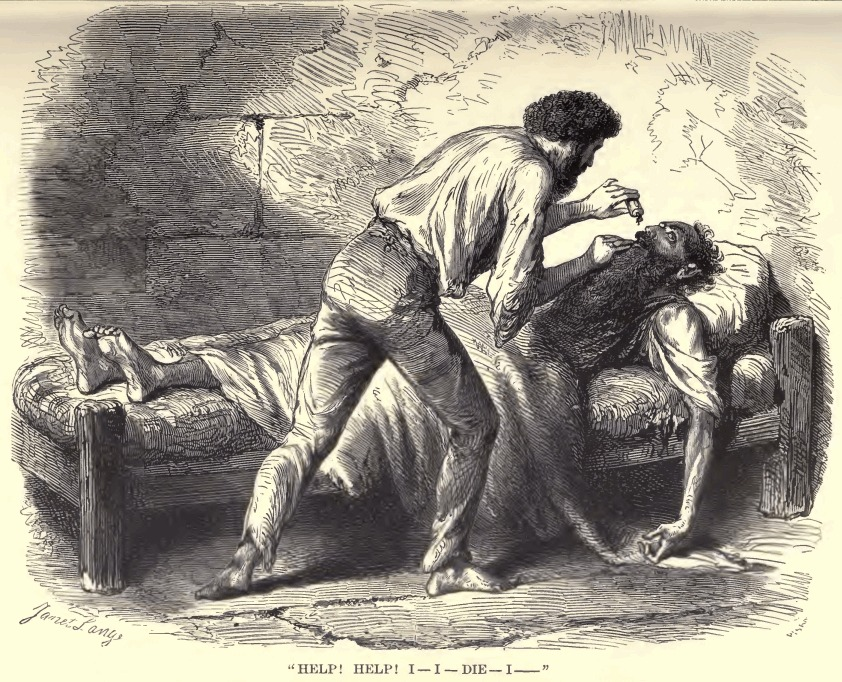
\includegraphics[width=\textwidth]{0229m.jpg}
\end{figure}

So sudden and violent was the fit that the unfortunate prisoner was
unable to complete the sentence; a violent convulsion shook his whole
frame, his eyes started from their sockets, his mouth was drawn on one
side, his cheeks became purple, he struggled, foamed, dashed himself
about, and uttered the most dreadful cries, which, however, Dantès
prevented from being heard by covering his head with the blanket. The
fit lasted two hours; then, more helpless than an infant, and colder
and paler than marble, more crushed and broken than a reed trampled
under foot, he fell back, doubled up in one last convulsion, and became
as rigid as a corpse.

Edmond waited till life seemed extinct in the body of his friend, then,
taking up the knife, he with difficulty forced open the closely fixed
jaws, carefully administered the appointed number of drops, and
anxiously awaited the result. An hour passed away and the old man gave
no sign of returning animation. Dantès began to fear he had delayed too
long ere he administered the remedy, and, thrusting his hands into his
hair, continued gazing on the lifeless features of his friend. At
length a slight color tinged the livid cheeks, consciousness returned
to the dull, open eyeballs, a faint sigh issued from the lips, and the
sufferer made a feeble effort to move.

“He is saved! he is saved!” cried Dantès in a paroxysm of delight.

The sick man was not yet able to speak, but he pointed with evident
anxiety towards the door. Dantès listened, and plainly distinguished
the approaching steps of the jailer. It was therefore near seven
o’clock; but Edmond’s anxiety had put all thoughts of time out of his
head.

The young man sprang to the entrance, darted through it, carefully
drawing the stone over the opening, and hurried to his cell. He had
scarcely done so before the door opened, and the jailer saw the
prisoner seated as usual on the side of his bed. Almost before the key
had turned in the lock, and before the departing steps of the jailer
had died away in the long corridor he had to traverse, Dantès, whose
restless anxiety concerning his friend left him no desire to touch the
food brought him, hurried back to the abbé’s chamber, and raising the
stone by pressing his head against it, was soon beside the sick man’s
couch. Faria had now fully regained his consciousness, but he still lay
helpless and exhausted on his miserable bed.

“I did not expect to see you again,” said he feebly, to Dantès.

“And why not?” asked the young man. “Did you fancy yourself dying?”

“No, I had no such idea; but, knowing that all was ready for flight, I
thought you might have made your escape.”

The deep glow of indignation suffused the cheeks of Dantès.

“Without you? Did you really think me capable of that?”

“At least,” said the abbé, “I now see how wrong such an opinion would
have been. Alas, alas! I am fearfully exhausted and debilitated by this
attack.”

“Be of good cheer,” replied Dantès; “your strength will return.” And as
he spoke he seated himself near the bed beside Faria, and took his
hands. The abbé shook his head.

“The last attack I had,” said he, “lasted but half an hour, and after
it I was hungry, and got up without help; now I can move neither my
right arm nor leg, and my head seems uncomfortable, which shows that
there has been a suffusion of blood on the brain. The third attack will
either carry me off, or leave me paralyzed for life.”

“No, no,” cried Dantès; “you are mistaken—you will not die! And your
third attack (if, indeed, you should have another) will find you at
liberty. We shall save you another time, as we have done this, only
with a better chance of success, because we shall be able to command
every requisite assistance.”

“My good Edmond,” answered the abbé, “be not deceived. The attack which
has just passed away, condemns me forever to the walls of a prison.
None can fly from a dungeon who cannot walk.”

“Well, we will wait,—a week, a month, two months, if need be,—and
meanwhile your strength will return. Everything is in readiness for our
flight, and we can select any time we choose. As soon as you feel able
to swim we will go.”

“I shall never swim again,” replied Faria. “This arm is paralyzed; not
for a time, but forever. Lift it, and judge if I am mistaken.”

The young man raised the arm, which fell back by its own weight,
perfectly inanimate and helpless. A sigh escaped him.

“You are convinced now, Edmond, are you not?” asked the abbé. “Depend
upon it, I know what I say. Since the first attack I experienced of
this malady, I have continually reflected on it. Indeed, I expected it,
for it is a family inheritance; both my father and grandfather died of
it in a third attack. The physician who prepared for me the remedy I
have twice successfully taken, was no other than the celebrated
Cabanis, and he predicted a similar end for me.”

\begin{figure}[ht]
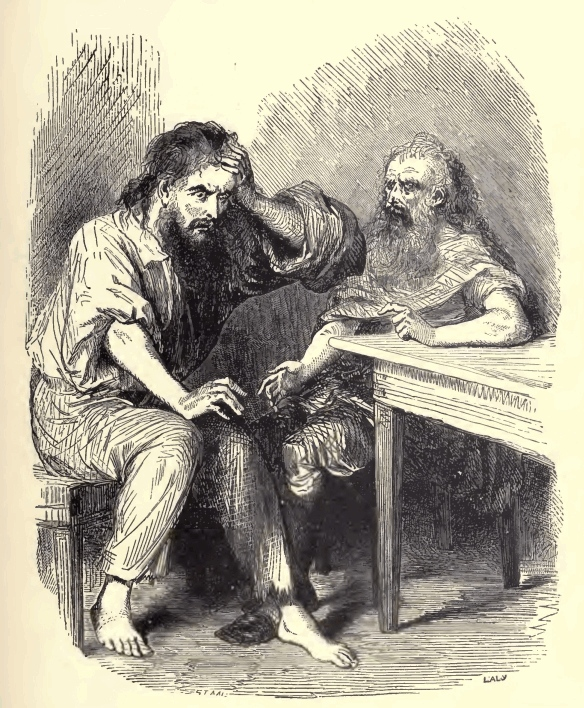
\includegraphics[width=\textwidth]{0233m.jpg}
\end{figure}

“The physician may be mistaken!” exclaimed Dantès. “And as for your
poor arm, what difference will that make? I can take you on my
shoulders, and swim for both of us.”

“My son,” said the abbé, “you, who are a sailor and a swimmer, must
know as well as I do that a man so loaded would sink before he had done
fifty strokes. Cease, then, to allow yourself to be duped by vain
hopes, that even your own excellent heart refuses to believe in. Here I
shall remain till the hour of my deliverance arrives, and that, in all
human probability, will be the hour of my death. As for you, who are
young and active, delay not on my account, but fly—go—I give you back
your promise.”

“It is well,” said Dantès. “Then I shall also remain.” Then, rising and
extending his hand with an air of solemnity over the old man’s head, he
slowly added, “By the blood of Christ I swear never to leave you while
you live.”

Faria gazed fondly on his noble-minded, single-hearted, high-principled
young friend, and read in his countenance ample confirmation of the
sincerity of his devotion and the loyalty of his purpose.

“Thanks,” murmured the invalid, extending one hand. “I accept. You may
one of these days reap the reward of your disinterested devotion. But
as I cannot, and you will not, quit this place, it becomes necessary to
fill up the excavation beneath the soldier’s gallery; he might, by
chance, hear the hollow sound of his footsteps, and call the attention
of his officer to the circumstance. That would bring about a discovery
which would inevitably lead to our being separated. Go, then, and set
about this work, in which, unhappily, I can offer you no assistance;
keep at it all night, if necessary, and do not return here tomorrow
till after the jailer has visited me. I shall have something of the
greatest importance to communicate to you.”

Dantès took the hand of the abbé in his, and affectionately pressed it.
Faria smiled encouragingly on him, and the young man retired to his
task, in the spirit of obedience and respect which he had sworn to show
towards his aged friend.
